\chapter{Derivations and calculations}
\label{MethodsAppendix}
\graphicspath{{Figures/MethodsAppendix/}{Figures/Common/}}

%Some content goes here.

% Perhaps this appendix might be called `technical details' or the like. And then we could cover things to keep an eye out for when doing simulations. Things like running off the edge of k-space causing phantom reflections, imaginary time algorithms. I could imagine quite a summary of techniques being possible.

\section{Example calculation of the momentum density flux}
\label{MethodsAppendix:MomentumDensityFluxExampleCalculation}

\begin{figure}
    \centering
    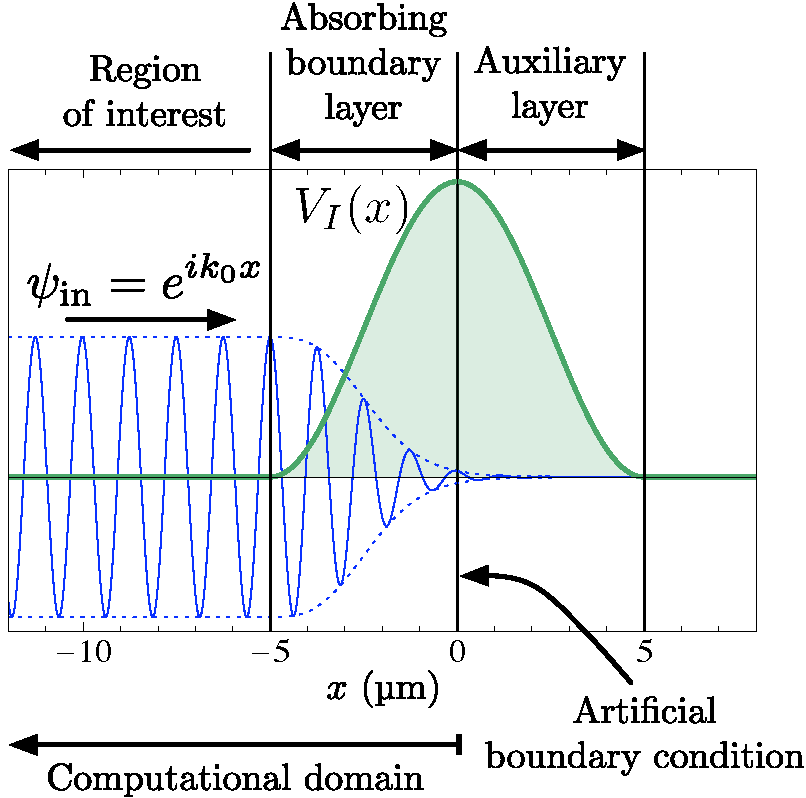
\includegraphics[width=8cm]{AbsorbingBoundaryLayerScattering}
    \caption{\label{MethodsAppendix:AbsorbingBoundaryLayerScattering} An incident wave of wavenumber $k_0$ incident on an absorbing boundary layer. The region of interest is the part of the computational domain in which the absorbing potential $V_I(x)$ is zero. An auxiliary layer is added outside of the absorbing boundary layer as a model for a number of artificial boundary conditions (see main text).}
\end{figure}

As a demonstration of the efficacy of the method described in \sectionref{Peaks:AbsorbingBoundaryTricks} for determining the rate of loss of momentum density from a region of space, we consider a wave of wavenumber $k_0$ incident from the left on an imperfect absorbing boundary layer in a 1D computational domain (see \figureref{MethodsAppendix:AbsorbingBoundaryLayerScattering}), and compare $\Phi(k, t)$ (refer to \eqref{Peaks:MomentumDensityFlux}) to the result expected in the case of a perfect absorbing boundary layer of $\displaystyle \frac{\hbar k_0}{M}\delta(k - k_0)$. In this example $s$-wave scattering will be neglected. As the computational domain in this example is effectively infinite, the wavefunction used in the evaluation of \eqref{Peaks:MomentumDensityFlux} will be restricted to be nonzero only in the absorbing boundary layer to demonstrate the finite momentum resolution obtainable from this method due to the (except in this example) finite extent of the computational domain.

As a model for a number of different artificial boundary conditions we consider there to be \emph{no} artificial boundary condition at the edge of the computational domain, and instead it to be surrounded by an `auxiliary layer' in which there is a negative imaginary potential the reflection of that in the absorbing boundary layer. The negative imaginary potential is then symmetric about the edge of the computational domain. In the case of periodic boundary conditions, the auxiliary layer will correspond to the absorbing boundary layer on the other side of the computational domain in which it is assumed that the reflected negative imaginary potential is used. In the case of Dirichlet or Neumann boundary conditions in which respectively the wavefunction or its derivative is set to zero on the boundary, the auxiliary layer corresponds to the absorbing boundary layer reflected. In either of these latter two cases, the wavefunction for the actual artificial boundary conditions will be a linear combination of the wavefunction \emph{without} the artificial boundary conditions in the absorbing boundary layer and in the auxiliary layer. Specifically, in the case of Dirichlet boundary conditions in which the wavefunction is set to zero on the boundary, the wavefunction in the presence of the artificial boundary condition $\psi_\text{abc}(\bm{x})$ will be given by $\psi_\text{abc}(\bm{x}) = \psi(\bm{x}) - \psi(-\bm{x})$ where $\psi(\bm{x})$ is the wavefunction in the absence of the artificial boundary condition, and $x=0$ corresponds to the edge of the computational domain.

To calculate $\Phi(k, t)$ from \eqref{Peaks:MomentumDensityFlux} it is necessary to know the solution $\psi(x)$ to the time-independent Schrödinger equation subject to the boundary conditions that there is an incident wave from the left with wavenumber $k_0$ and no incident wave from the right. Given two linearly independent solutions to the Schrödinger equation in the doubled absorbing boundary layer (the absorbing boundary layer / auxiliary layer region), $\psi(x)$ can be found by applying these boundary conditions. It now remains to obtain two linearly independent solutions to the time-independent Schrödinger equation within the doubled absorbing boundary layer.

Solutions to the time-independent Schrödinger equation within the doubled absorbing boundary layer can be obtained with relative ease in one dimension as it is simply an ordinary differential equation,
\begin{align}
    -\frac{\hbar^2}{2M}\frac{d^2 \psi}{dx^2} + V(x) \psi(x) &= E(k_0) \psi(x) = \frac{\hbar^2 k_0^2}{2M} \psi(x),
\end{align}
which is equivalent to
\begin{align}
    \frac{d^2 \psi}{dx^2} &= \frac{2 M}{\hbar^2} V(x) \psi(x) - k_0^2 \psi(x).
    \label{MethodsAppendix:1DTimeIndependentSchrodingerEquation}
\end{align}
Two linearly independent (but not necessarily orthogonal) solutions $\phi_1(x)$, $\phi_2(x)$ to \eqref{MethodsAppendix:1DTimeIndependentSchrodingerEquation} can be found by simply choosing two linearly independent initial conditions and numerically propagating the solutions through the potential $V(x) = -i V_I(x)$. The solution $\psi(x) = c_1 \phi_1(x) + c_2 \phi_2(x)$ can then be found by requiring continuity of the wavefunction and its derivative at the left and right edges of the doubled absorbing boundary layer,
\begin{subequations}
    \label{MethodsAppendix:1DBoundaryConditions}
    \begin{align}
        e^{i k x} + \alpha_R e^{-i k x} \Big|_\text{left} &=  c_1 \phi_1(x) + c_2 \phi_2(x) \Big|_\text{left}, \\
        \frac{d}{dx}\big( e^{i k x} + r e^{-i k x}\big) \Big|_\text{left} &=  \frac{d}{dx} \big( c_1 \phi_1(x) + c_2 \phi_2(x) \big) \Big|_\text{left},\\
        \alpha_T e^{i k x} \Big|_\text{right} &= c_1 \phi_1(x) + c_2 \phi_2(x) \Big|_\text{right}, \\
        \frac{d}{dx} \big( \alpha_T e^{i k x} \big) \Big|_\text{right} &= \frac{d}{dx} \big( c_1 \phi_1(x) + c_2 \phi_2(x) \big) \Big|_\text{right},
    \end{align}
\end{subequations}
where $\alpha_R$ and $\alpha_T$ are the reflected and transmitted amplitudes respectively. 

As a by-product of solving \eqref{MethodsAppendix:1DBoundaryConditions} for $\psi(x)$, the reflection and transmission fractions $R=\abs{\alpha_R}^2$ and $T=\abs{\alpha_T}^2$ respectively can be obtained, giving a quantitative description of the effectiveness of a given absorbing boundary layer. For reflecting artificial boundary conditions, the reflection coefficient is $R'= \abs{\alpha_R \mp \alpha_T}^2$ respectively for Dirichlet and Neumann boundary conditions, and as $\alpha_R$ and $\alpha_T$ can not both be significant simultaneously for any absorbing boundary layer that is effective over some finite range of wavenumbers, the approximation $R' \approx \max(R, T)$ can be used.  Hence $R$ and $T$ are useful measures of the effectiveness of an absorbing boundary layer independent of the artificial boundary conditions used.

\begin{figure}
    \centering
    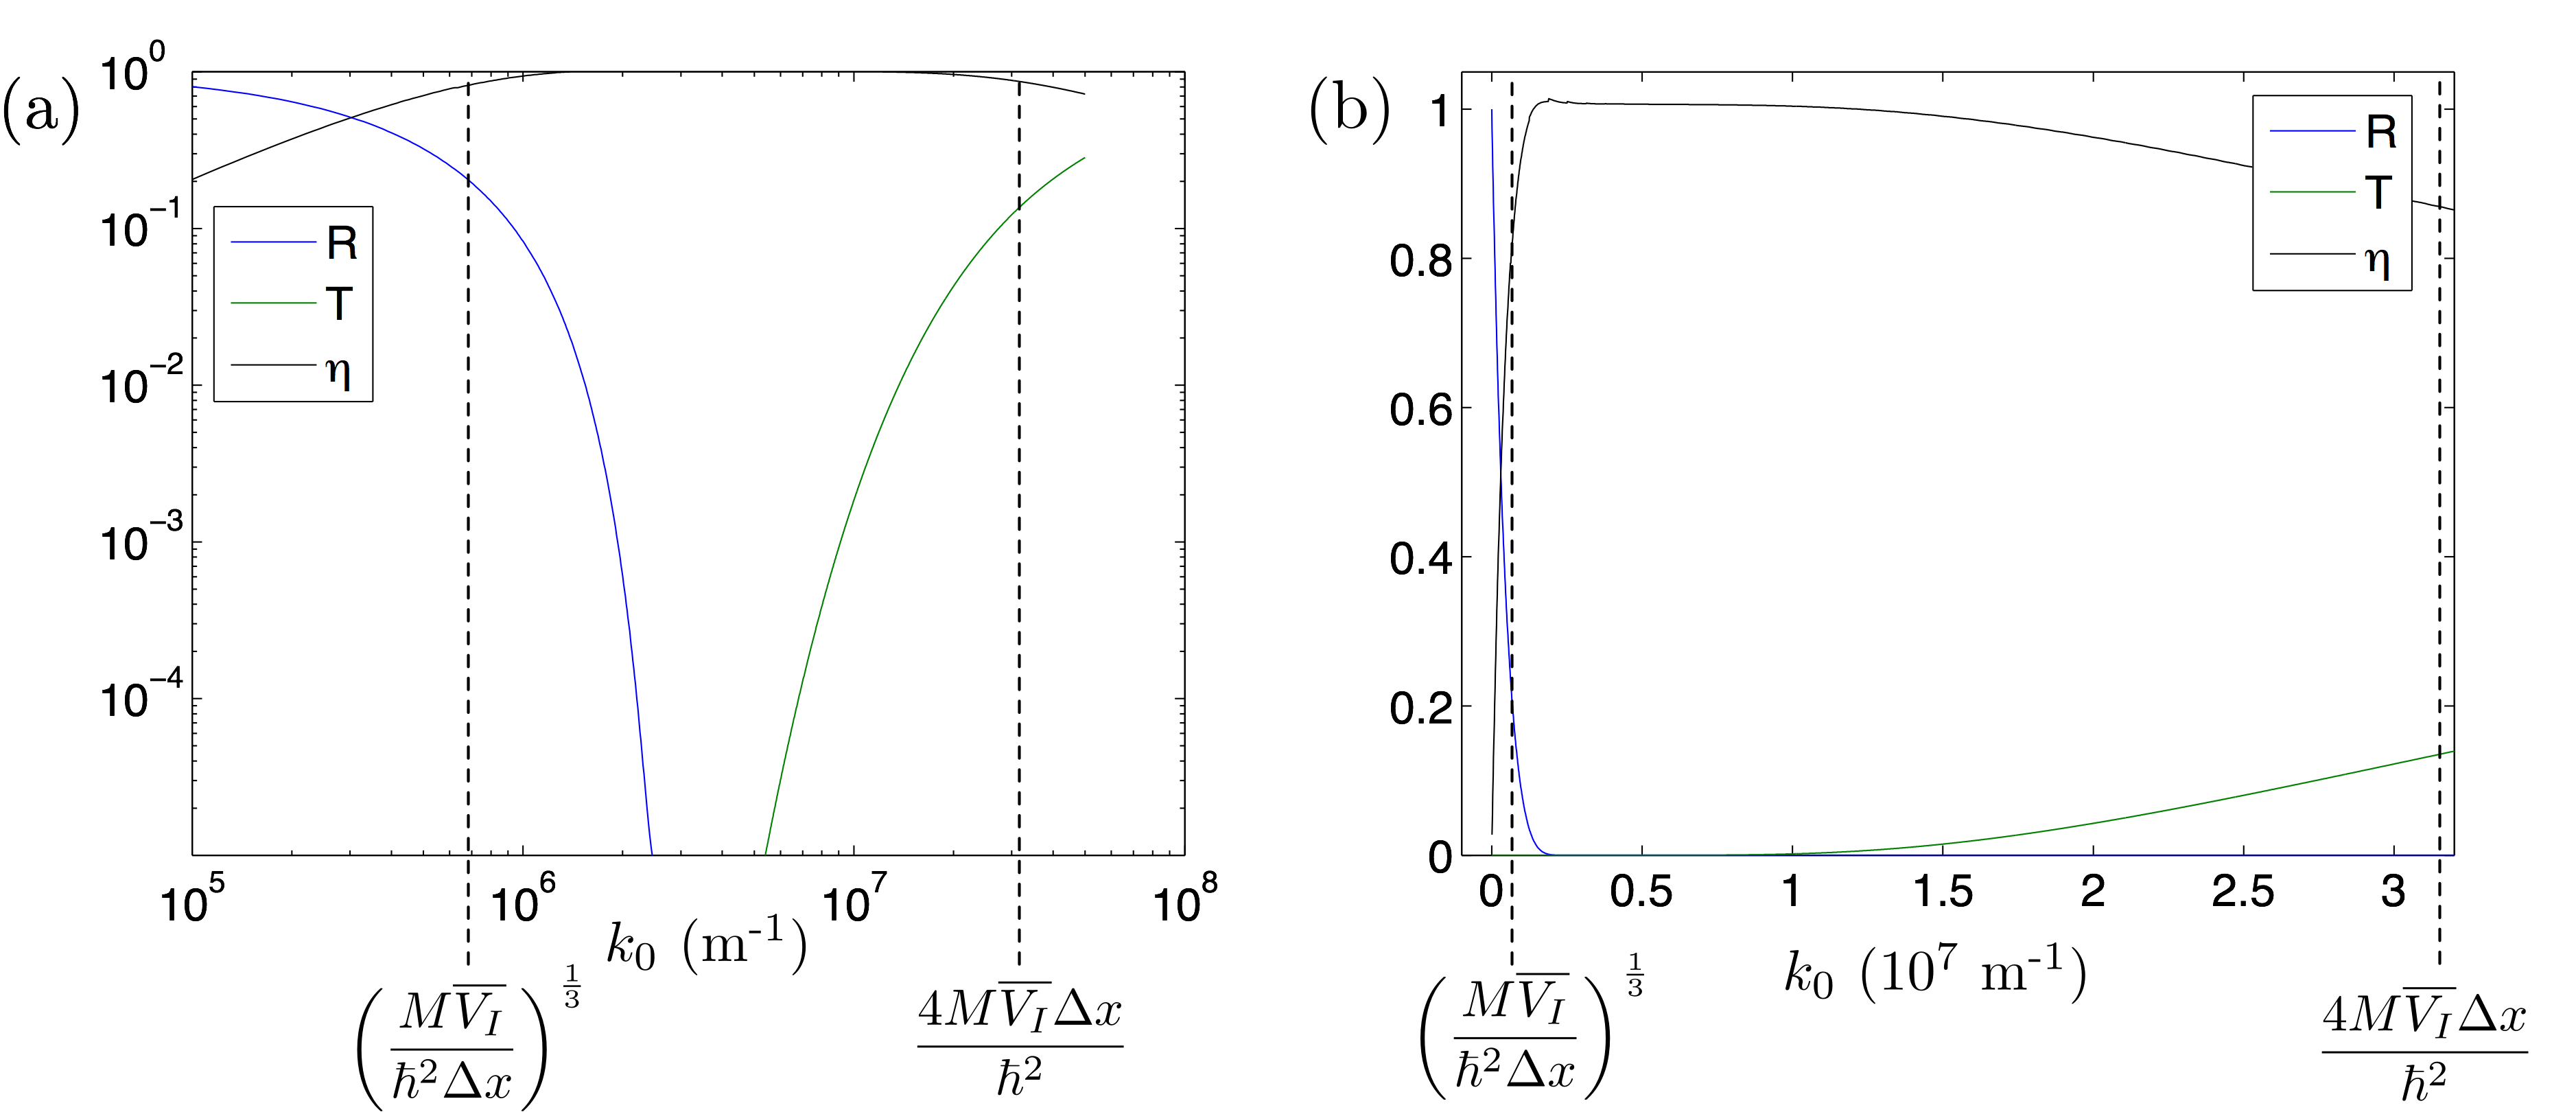
\includegraphics[width=14cm]{AbsorbingBoundaryLayerEffectiveness}
    \caption{\label{MethodsAppendix:AbsorbingBoundaryLayerEffectiveness} The reflection $R$ and transmission $T$ coefficients from a typical absorbing boundary layer as a function of wavenumber. The potential used was $\displaystyle V_I(x) = \hbar \omega \cos^2\left( \frac{\pi x}{2 \Delta x} \right)$ where $\omega = \unit[5 \times 10^4]{rad.s\textsuperscript{-1}}$ and $\Delta x = \unit[5]{\micro m}$ is the size of the absorbing boundary layer. Also marked on this figure are the approximate lower and upper bounds of the effectiveness of the absorbing boundary layer as given by \eqref{BackgroundTheory:AbsorbingBoundaryKEffectiveRange}.}
\end{figure}

In \figureref{MethodsAppendix:AbsorbingBoundaryLayerEffectiveness} the reflected and transmitted fractions $R$ and $T$ are plotted as a function of the incident wavenumber and a comparison is made to the approximate range of validity of the absorbing boundary as given by \eqref{BackgroundTheory:AbsorbingBoundaryKEffectiveRange}. 


With $\psi(x)$ determined, the steady state momentum density flux $\Phi_{k_0}(k)$ can be obtained for a given incident wavenumber $k_0$. This distribution is plotted in \figureref{MethodsAppendix:PhiAccuracy} for the same absorbing boundary used in \figureref{MethodsAppendix:PhiAccuracy}. As any real absorbing boundary layer will have finite extent, the resolution of $\Phi_{k_0}(k)$ will be limited by $\Delta k = \pi/\Delta x$, where $\Delta x$ is the width of the absorbing boundary layer. This finite resolution will prevent $\Phi_{k_0}(k)$ reproducing the exact result in the limit of a perfect absorbing boundary layer of $\displaystyle \frac{\hbar k_0}{M}\delta(k - k_0)$. As a measure of the accuracy of $\Phi_{k_0}(k)$, its integral over a range of a few $\Delta k$ should be compared to the exact answer. To this aim we define
\begin{align}
    \eta(k_0) &= \left(\frac{\hbar k_0}{M}\right)^{-1} \int_{k_0-5\Delta k}^{k_0 + 5\Delta k} dk\, \Phi_{k_0}(k),
\end{align}
where $\eta(k_0)$ is plotted in \figureref{MethodsAppendix:AbsorbingBoundaryLayerEffectiveness}. As expected, $\eta \approx 1$ over the same range of incident wavenumbers for which the absorbing boundary layer is effective.

\begin{figure}
    \centering
    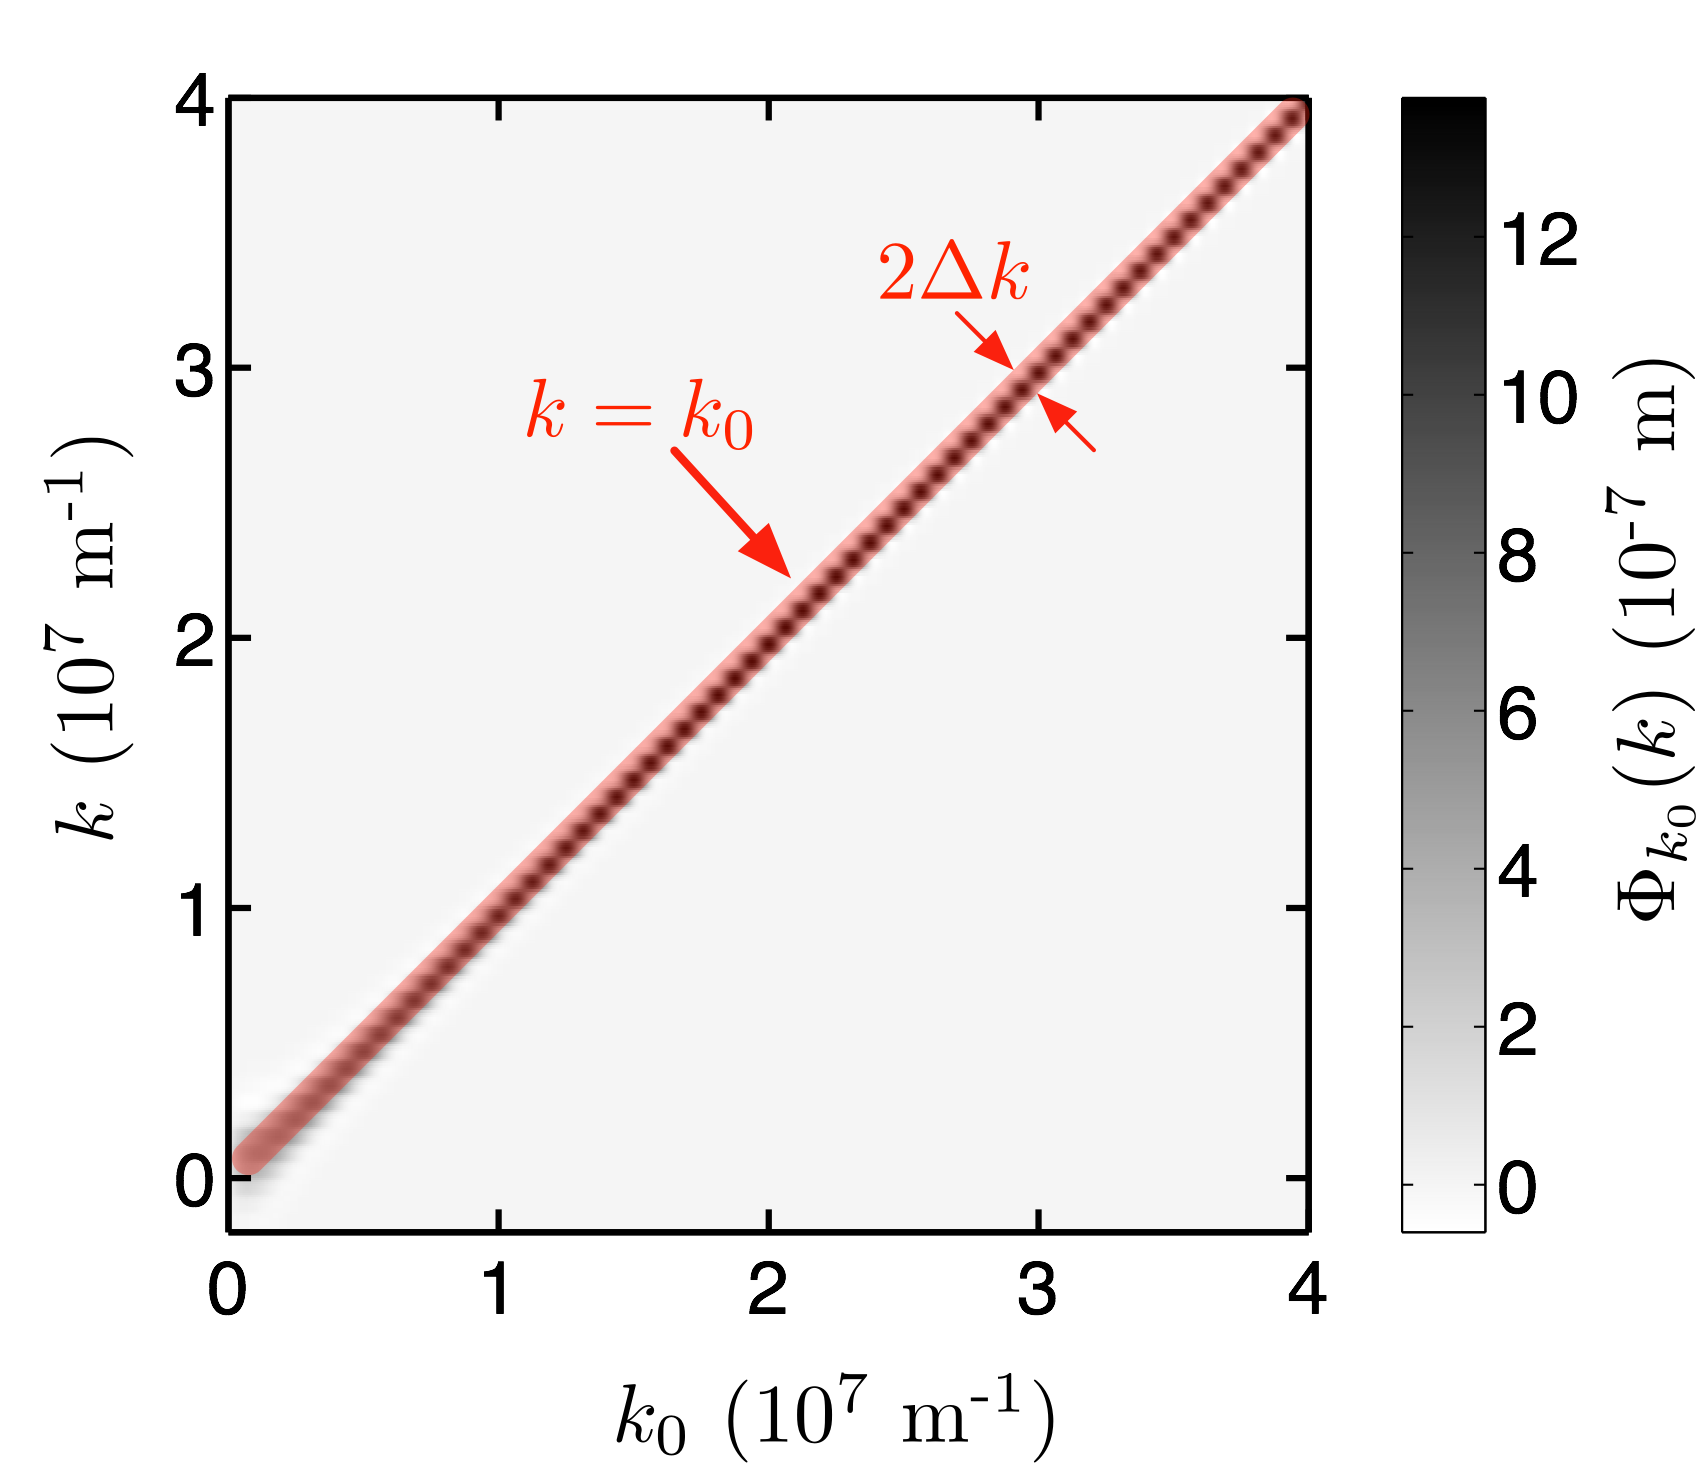
\includegraphics[width=8cm]{PhiAccuracy}
    \caption{\label{MethodsAppendix:PhiAccuracy} The momentum flux density $\Phi_{k_0}(k)$ leaving the region of interest in \figureref{MethodsAppendix:AbsorbingBoundaryLayerScattering} as a function of the incident wavenumber $k_0$. As expected, $\Phi_{k_0}(k)$ is sharply peaked around $k=k_0$. The resolution of $\Phi_{k_0}(k)$, $\Delta k$ is indicated by the width of the $k=k_0$ line.}
\end{figure}

\section[Solving the Quantum Kinetic Theory model]{Solving the Quantum Kinetic Theory model of \chapterref{KineticTheory}}
\label{MethodsAppendix:KineticTheory}

One of the difficulties involved in solving the kinetic model of \chapterref{KineticTheory} is that the energy range that the problem is defined over changes in time.  The maximum energy is simply the energy of the evaporative cut-off $\varepsilon_\text{cut}$, while the minimum energy is the chemical potential of the condensate $\mu(t)$.  A discretisation of the energy dimension over the range $[0, \varepsilon_\text{cut}]$ will suffer from problems accurately representing the lower-end of the distribution where the minimum energy of the thermal atoms is varying.  An alternative is write the problem in terms of a shifted energy coordinate $\overline{\varepsilon} \equiv \varepsilon - \mu(t)$ so that the minimum energy of the system is now fixed.  Of course the same problem now exists at the upper end of the energy range where the maximum energy $\overline{\varepsilon}_\text{max} = \varepsilon_\text{cut} - \mu(t)$ is now time-dependent.  However, at equilibrium there will be significantly fewer thermal atoms at the evaporation cut-off than there will be near the condensate (this is illustrated in \figureref{KineticTheory:EnergyDistributionFunctionEvolution}(a)).  This choice will then result in smaller numerical errors than the alternative.

Written in terms of the shifted energy variable $\overline{\varepsilon}$, the contribution due to the replenishment is
\begin{align}
    \left. \frac{\partial\big(\overline{\rho}(\overline{\varepsilon}, t) \overline{g}(\overline{\varepsilon}, t)\big)}{\partial t}\right|_\text{replenishment} &= \Gamma \overline{\rho}_0(\overline{\varepsilon}) \overline{g}_T(\overline{\varepsilon}),
    \label{MethodsAppendix:KineticTheory:ReplenishmentProcess}
\end{align}
where a bar over a function is used to indicate that it is defined in terms of the shifted energy coordinate.  The original form of this term is given by \eqref{KineticTheory:ReplenishmentProcess}.

\subsection{Density of states}
\label{MethodsAppendix:QKTDensityOfStates}

Although the evolution equations for the kinetic model \eqref{KineticTheory:EvolutionEquations} are written in terms of the product of the density of states $\rho(\varepsilon, t)$ and the energy distribution function $g(\varepsilon, t)$, it will be necessary to separately determine the energy distribution function to evaluate the collisional contributions given in the following section. To extract the energy distribution function it is necessary to have an explicit expression for the density of states for the thermal cloud. This density of states is not simply the same as that for a harmonic trap as the thermal modes will experience a mean-field repulsion due to the condensate mode. The effective potential experienced by the thermal atoms is
\begin{align}
    V_\text{eff}(\bm{r}, t) &= V_\text{trap}(\bm{r}) + 2 g n_c(\bm{r}, t), \label{MethodsAppendix:QKTEffectivePotential}
\end{align}
where $V_\text{trap}(\bm{r})$ is the potential due to the magnetic trap, $g = 4\pi \hbar^2 a/m$, $a$ is the s-wave scattering length and $n_c(\bm{r}, t)$ is the condensate density which was assumed to follow a Thomas-Fermi distribution in \chapterref{KineticTheory}.  Note that the `2' in the above expression is the full Hartree-Fock mean field experienced by the thermal atoms (see \eqref{Peaks:ThermalParticleEnergySpectrum}, or \citep[Chapter 8]{PethickSmith} for further details) which is twice the mean-field repulsion experienced by condensate atoms.  This is essentially due to the thermal atoms being distinguishable from the condensate atoms, while the condensate atoms are indistinguishable from one another.

The density of states in the presence of the effective potential \eqref{MethodsAppendix:QKTEffectivePotential} is given by
\begin{align}
    \rho(\varepsilon, t) &= \int \frac{d \bm{r}\, d \bm{p}}{(2\pi \hbar)^3} \,\delta\left(\varepsilon - V_\text{eff}(\bm{r}, t) - \bm{p}^2/2 m\right).
    \label{MethodsAppendix:DensityOfStatesDefinition}
\end{align}
The integrals are performed in \citep{Bijlsma:2000} giving the following result in terms of the shifted energy coordinate (Eqs.~49 and 50 in \citep{Bijlsma:2000})
\begin{align}
    \overline{\rho}(\overline{\varepsilon}, t) &= \frac{2}{\pi \hbar \overline{\omega}} \left[I_-(\overline{\varepsilon}) + I_+(\overline{\varepsilon})\right],
\end{align}
where the functions $I_\pm(\overline{\varepsilon})$ are
\begin{align}
    I_-(\overline{\varepsilon}) &= \left.\frac{u_-^3 x}{4} - \frac{a_- u_- x}{8} - \frac{a_-^2}{8}\ln(x + u_-)\right|_{x=\sqrt{\max\{0, -a_-\}}}^{x=\sqrt{2\mu/\hbar \overline{\omega}}}, \label{MethodsAppendix:QKTIMinus}\\
    I_+(\overline{\varepsilon}) &= \left.- \frac{u_+^3 x}{4} + \frac{a_+ u_+ x}{8} + \frac{a_+^2}{8} \arcsin\left(\frac{x}{\sqrt{a_+}}\right)\right|_{x=\sqrt{2\mu/\hbar\overline{\omega}}}^{x=\sqrt{a_+}}, \label{MethodsAppendix:QKTIPlus}
\end{align}
with $a_\pm = 2(\overline{\varepsilon}\pm \mu)/\hbar\overline{\omega}$, and $u_\pm = \sqrt{a_\pm \mp x^2}$. Note that there is a minor typo in \citet{Bijlsma:2000}, the lower limit of $I_-(\overline{\varepsilon})$ is given as $x=\sqrt{\max\{0, a_-\}}$, while it should read $x=\sqrt{\max\{0, -a_-\}}$ as in \eqref{MethodsAppendix:QKTIMinus}.

\subsection{Collision and energy-redistribution in Quantum Kinetic Theory}
\label{MethodsAppendix:QKTOtherTerms}

The forms of the collision and energy-redistribution terms of the kinetic model described in \chapterref{KineticTheory} were omitted there for sake of clarity as their derivation was not part of the work presented there.  A full derivation of these terms is given in \citep{Bijlsma:2000,Proukakis:2008}.

The contribution due to thermal--thermal collisions is given in Eq.~26 of \citep{Bijlsma:2000} and has the form
\begin{align}
    \begin{split}
        \left. \frac{\partial\big(\overline{\rho}(\overline{\varepsilon}_1, t) \overline{g}(\overline{\varepsilon}_1, t)\big)}{\partial t}\right|_\text{thermal--thermal} &= \frac{m^3 g^2}{2 \pi^3 \hbar^7} \int d\overline{\varepsilon}_2 \int d\overline{\varepsilon}_3 \int d\overline{\varepsilon}_4 \,\overline{\rho}(\overline{\varepsilon}_\text{min}, t)\\
        &\relphantom{=} \times\delta(\overline{\varepsilon}_1 + \overline{\varepsilon}_2 - \overline{\varepsilon}_3 - \overline{\varepsilon}_4) \\
        &\relphantom{=} \times [ (1+\overline{g}_1) (1+\overline{g}_2) \overline{g}_3 \overline{g}_4 - \overline{g}_1 \overline{g}_2 (1+\overline{g}_3) (1+\overline{g}_4)],
    \end{split}
\end{align}
where $\overline{\varepsilon}_\text{min}$ is the minimum of the $\overline{\varepsilon}_i$, and $\overline{g}_i = \overline{g}(\overline{\varepsilon}_i, t)$. 

The contribution due to thermal--condensate collisions is given by Eq.~53 and Eq.~58--60 of \citep{Bijlsma:2000} and has the form
\begin{align}
    \begin{split}
        \left. \frac{\partial\big(\overline{\rho}(\overline{\varepsilon}_1, t) \overline{g}(\overline{\varepsilon}_1, t)\big)}{\partial t}\right|_\text{thermal--condensate} &= \frac{m^3 g^2}{2 \pi^3 \hbar^7} \int d \overline{\varepsilon}_2 \int d\overline{\varepsilon}_3 \int d\overline{\varepsilon}_4 \,\delta(\overline{\varepsilon}_2 - \overline{\varepsilon}_3 - \overline{\varepsilon}_4)\\
        &\relphantom{=}\times\left[ \delta(\overline{\varepsilon}_1 - \overline{\varepsilon}_2) - \delta(\overline{\varepsilon}_1 - \overline{\varepsilon}_3) - \delta(\overline{\varepsilon}_1- \overline{\varepsilon}_4)\right]\\
        &\relphantom{=} \times \left[(1+\overline{g}_2)\overline{g}_3 \overline{g}_4 - \overline{g}_2 (1+\overline{g}_3)(1+\overline{g}_4) \right]\\
        &\relphantom{=}\times  \int_{\overline{U}_\text{eff}(\bm{r}, t) \leq \overline{U}_-} d \bm{r}\, n_c(\bm{r}, t),
    \end{split}
    \label{MethodsAppendix:QKTRhoGThermalCondensateEvolution}
\end{align}
where $\displaystyle \overline{U}_- = \frac{2}{3}\left[(\overline{\varepsilon}_3 + \overline{\varepsilon}_4)-\sqrt{\overline{\varepsilon}_3^2 - \overline{\varepsilon}_3 \overline{\varepsilon}_4 + \overline{\varepsilon}_4^2}\right]$, and $\overline{U}_\text{eff}(\bm{r}, t) = U_\text{eff}(\bm{r}, t) - \mu(t)$.
The corresponding contribution to the evolution of the condensate number is simply
\begin{align}
    \left. \frac{d N_0}{d t}\right|_\text{thermal--condensate} &= - \int d\overline{\varepsilon} \,\left. \frac{\partial\big(\overline{\rho}(\overline{\varepsilon}, t) \overline{g}(\overline{\varepsilon}, t)\big)}{\partial t}\right|_\text{thermal--condensate}.
    \label{MethodsAppendix:QKTNThermalCondensateEvolution}
\end{align}


Finally, the contribution due to energy redistribution is (Eqs.~32 and 52 in \citep{Bijlsma:2000})
\begin{align}
    \left. \frac{\partial\big(\overline{\rho}(\overline{\varepsilon}_1, t) \overline{g}(\overline{\varepsilon}_1, t)\big)}{\partial t}\right|_\text{redistribution} &= - \frac{\partial \big( \overline{\rho}_\text{w} \overline{g}\big)}{\partial \overline{\varepsilon}},
    \label{MethodsAppendix:QKTRedistributionEvolution}
\end{align}
where $\overline{\rho}_\text{w}$ is the weighted density of states
\begin{align}
    \overline{\rho}_\text{w}(\overline{\varepsilon}) &= \frac{2}{\pi \hbar \overline{\omega}} \left[ I_-(\overline{\varepsilon}) - I_+(\overline{\varepsilon})\right] \frac{d \mu}{dt},
\end{align}
where the functions $I_\pm(\overline{\varepsilon})$ are given in \eqref{MethodsAppendix:QKTIMinus} and \eqref{MethodsAppendix:QKTIPlus}.


\subsection{Three-body loss in Quantum Kinetic Theory}
\label{MethodsAppendix:QKT3BodyLoss}

The dominant density-dependent loss process in Bose-Einstein condensates is three-body loss \citep{Burt:1997fk,Soding:1999}. In \chapterref{KineticTheory} it was argued that three-body loss was an important process in the operation of the pumped atom laser scheme proposed there.  The following derivation of the three-body loss contribution to the kinetic model \eqref{KineticTheory:EvolutionEquations} was performed by \emph{Matthew Davis} and is presented for completeness.

Three-body loss (or three-body recombination) is the process in which three atoms collide forming a bound dimer with the third necessary to ensure both energy and momentum conservation.  The binding energy is sufficient to give the products of a three-body recombination process sufficient kinetic energy to rapidly escape the trap.  Three-body loss is then well-described by the master equation term
\begin{align}
    \left. \frac{d \hat{\rho}}{d t}\right|_\text{3-body loss} &= \frac{1}{3}L_3 \int d \bm{x} \,\mathcal{D} \left[ \hat{\Psi}^3(\bm{x}) \right] \hat{\rho},
    \label{MethodsAppendix:ThreeBodyLossMasterEquationTerm}
\end{align}
where $\mathcal{D}[\hat{c}]\hat{\rho} = \hat{c}\hat{\rho} \hat{c}^\dagger - \frac{1}{2}(\hat{c}^\dagger \hat{c}\hat{\rho} + \hat{\rho} \hat{c}^\dagger \hat{c})$ is the usual decoherence superoperator, and $L_3 = \unit[5.8\times 10^{-30}]{cm\textsuperscript{6}s\textsuperscript{-1}}$ \citep{Burt:1997fk} is the three-body recombination loss rate constant.  This equation, first derived by \citep{Jack:2002} has the familiar form of a decoherence superoperator with the state undergoing loss as the argument (cf. \sectionref{PenningIonisationAppendix:MasterEquation}). %This is a reasonable approximation as three-body recombination couples the state $\hat{\Psi}^3$ to a state that is rapidly depopulated.

The loss rate of atoms from the system due to three-body loss is readily obtained from \eqref{MethodsAppendix:ThreeBodyLossMasterEquationTerm} as
\begin{align}
    \left.\frac{d N}{dt} \right|_\text{3-body loss} &=  \Tr\left\{\int d \bm{r}\,\hat{\Psi}^\dagger(\bm{r})\hat{\Psi}(\bm{r}) \left.\frac{d \hat{\rho}}{dt}\right|_\text{3-body loss} \right\} = - L_3 \int d \bm{r}\, \mean{\hat{\Psi}^\dagger(\bm{r})^3 \hat{\Psi}(\bm{r})^3}.
    \label{MethodsAppendix:ThreeBodyLossNumberLossRate}
\end{align}

To separate the contributions to \eqref{MethodsAppendix:ThreeBodyLossNumberLossRate} due to the thermal and condensed components, we use an approach similar to that of the Bogoliubov theory discussed in \sectionref{Peaks:ElementaryExcitations}.  We write the annihilation operator $\hat{\Psi}$ in terms of its mean value $\Psi \equiv \mean{\hat{\Psi}}$ and the deviation operator $\delta \hat{\Psi} \equiv \hat{\Psi} - \Psi$ and substitute this into \eqref{MethodsAppendix:ThreeBodyLossNumberLossRate}.  In contrast to \sectionref{Peaks:ElementaryExcitations} in which the zero-temperature limit was considered, the deviation operator defined here represents thermal fluctuations, which cannot be considered to be small.  Higher powers of $\delta\hat{\Psi}$ can therefore not be neglected.  However, thermal fluctuations have no well-defined phase relationship to one another or to the condensate.  Expectation values containing an unequal number of creation and annihilation deviation operators such as $\mean{\delta\hat{\Psi}\delta\hat{\Psi}}$ can therefore be assumed to be zero (cf. \eqref{Peaks:HamiltonianPowerSeriesQuadraticTerm} in which the $\delta\hat{\Psi}^\dagger \delta\hat{\Psi}^\dagger$ and $\delta\hat{\Psi}\delta\hat{\Psi}$ terms were retained as there is a well-defined phase relationship between the quasiparticles and the condensate).

Performing the substitution described, \eqref{MethodsAppendix:ThreeBodyLossNumberLossRate} becomes
\begin{align}
    \begin{split}
        \left.\frac{d N}{dt} \right|_\text{3-body loss} &=  -L_3 \int d \bm{r}\, \Big\{[n_c(\bm{r})]^3 + 9 [n_c(\bm{r})]^2 \mean{\delta\hat{\Psi}^\dagger(\bm{r}) \delta\hat{\Psi}(\bm{r})}\\
        &\relphantom{=-L_3 \int d \bm{r}\,\Big\{} + 9 n_c(\bm{r}) \mean{\delta\hat{\Psi}^\dagger(\bm{r})^2 \delta\hat{\Psi}(\bm{r})^2} + \mean{\delta\hat{\Psi}^\dagger(\bm{r})^3 \delta\hat{\Psi}(\bm{r})^3}\Big\},
    \end{split}
    \label{MethodsAppendix:ThreeBodyLossNumberLossRateInTermsOfDeviationOperators}
\end{align}
where $n_c(\bm{r}) = \abs{\Psi(\bm{r})}^2$ is the condensate density.

The non-condensate density is given by $n_T(\bm{r}) = \mean{\delta\hat{\Psi}^\dagger(\bm{r}) \delta\hat{\Psi}(\bm{r})}$.  As thermal states are Gaussian, the higher-order expectation values in the previous expression may be simplified by the application of Wick's theorem \citep{Wick:1950} giving
\begin{align}
    \mean{\delta\hat{\Psi}^\dagger(\bm{r})^2 \delta\hat{\Psi}(\bm{r})^2} &= 2 [n_T(\bm{r})]^2, \\
    \mean{\delta\hat{\Psi}^\dagger(\bm{r})^3 \delta\hat{\Psi}(\bm{r})^3} &= 6 [n_T(\bm{r})]^3.
\end{align}
Substituting these expressions back into \eqref{MethodsAppendix:ThreeBodyLossNumberLossRateInTermsOfDeviationOperators} yields
\begin{align}
    \left.\frac{d N}{dt} \right|_\text{3-body loss} &=  -L_3 \int d \bm{r}\, [n_c(\bm{r})]^3 + 9 [n_c(\bm{r})]^2 n_T(\bm{r}) + 18 n_c(\bm{r}) [n_T(\bm{r})]^2 + 6 [n_T(\bm{r})]^3.
    \label{MethodsAppendix:ThreeBodyLossNumberLossRateInTermsOfDensities}
\end{align}

The evaluation of this loss rate requires the evaluation of the condensate and thermal densities.  The condensate density $n_c(\bm{r})$ is fully determined by the condensate occupation $N_0(t)$ within the Thomas-Fermi approximation that has already been made elsewhere in the derivation of the kinetic model.  The first term of \eqref{MethodsAppendix:ThreeBodyLossNumberLossRateInTermsOfDensities} only involves the condensate density and may be evaluated analytically
\begin{align}
    \frac{d N_0}{dt} &= - L_3 \frac{15^{4/5}}{168 \pi^2} \left(\frac{m \overline{\omega}}{\hbar \sqrt{a}} \right)^{12/5} N_0^{9/5}.
\end{align}
The remaining terms of \eqref{MethodsAppendix:ThreeBodyLossNumberLossRateInTermsOfDensities} require an expression for the thermal density $n_T(\bm{r})$, which can be obtained from the energy distribution function $g(\varepsilon)$ and the density of states $\rho(\varepsilon)$.

The total number of thermal atoms $N_T$ can be written as
\begin{align}
    N_T &= \int d\varepsilon\, \rho(\varepsilon) g(\varepsilon),
    \label{MethodsAppendix:NThermalDefinition}
\end{align}
where the density of states is defined by \eqref{MethodsAppendix:DensityOfStatesDefinition}.  Substituting this into \eqref{MethodsAppendix:NThermalDefinition} and rearranging the order of integrals gives
\begin{align}
    N_T &= \int d \bm{r}\, \int d\varepsilon\, \rho(\varepsilon, \bm{r}) g(\varepsilon),
    \label{MethodsAppendix:NThermalInTermsOfRhoER}
\end{align}
where we have defined
\begin{align}
    \rho(\varepsilon, \bm{r}) &= \int d \bm{p}\, \delta\left(\varepsilon - V_\text{eff}(\bm{r}, t) - \bm{p}^2/2m\right) = \frac{m^{3/2}}{\sqrt{2} \pi^2 \hbar^3} \sqrt{\varepsilon - V_\text{eff}(\bm{r})}.
\end{align}
The thermal density can be identified from \eqref{MethodsAppendix:NThermalInTermsOfRhoER}
\begin{align}
    n_T(\bm{r}) &= \int d\varepsilon\, \rho(\varepsilon, \bm{r}) g(\varepsilon).
    \label{MethodsAppendix:nThermalInTermsOfRhoER}
\end{align}

The remaining terms of \eqref{MethodsAppendix:ThreeBodyLossNumberLossRateInTermsOfDensities} can now be expressed in terms of the energy distribution function $g(\varepsilon)$ and the density of states $\rho(\varepsilon)$ by substituting \eqref{MethodsAppendix:nThermalInTermsOfRhoER} for one of the factors of $n_T(\bm{r})$ in each term
\begin{align}
    -L_3 \int d \bm{r}\, 9 [n_c(\bm{r})]^2 n_T(\bm{r}) &= - L_3 \int d\varepsilon\, g(\varepsilon) \int d \bm{r}\, 9 \rho(\varepsilon, \bm{r}) [n_c(\bm{r})]^2, \label{MethodsAppendix:Condensate2Thermal1}\\
    -L_3 \int d \bm{r}\, 18 n_c(\bm{r}) [n_T(\bm{r})]^2 &= - L_3 \int d\varepsilon\, g(\varepsilon) \int d \bm{r}\, 18 \rho(\varepsilon, \bm{r}) n_c(\bm{r}) n_T(\bm{r}), \label{MethodsAppendix:Condensate1Thermal2}\\
    -L_3 \int d \bm{r}\, 6 [n_T(\bm{r})]^3 &= - L_3 \int d\varepsilon\, g(\varepsilon) \int d \bm{r}\, 6 \rho(\varepsilon, \bm{r}) [n_T(\bm{r})]^2. \label{MethodsAppendix:Condensate0Thermal3}
\end{align}
From these expressions the rate of loss of atoms of energy $\varepsilon$ from the distribution can be identified
\begin{align}
    \left.\frac{\partial\big(\rho(\varepsilon) g(\varepsilon)\big)}{\partial t}\right|_\text{3-body loss} &= -L_3 \int d \bm{r}\, \rho(\varepsilon, \bm{r}) g(\varepsilon) \left\{ 3 [n_c(\bm{r})]^2 + 12 n_c(\bm{r}) n_T(\bm{r}) + 6 [n_T(\bm{r})]^2 \right\},
    \label{MethodsAppendix:QKT3BodyLossDistributionEvolution}
\end{align}
where the contributions due to the terms involving only one or two thermal atoms have been multiplied by $1/3$ and $2/3$ respectively to share appropriately the total loss.  The corresponding term for the condensate number evolution is
\begin{align}
    \begin{split}
        \left. \frac{d N_0}{dt} \right|_\text{3-body loss} &= - L_3 \frac{15^{4/5}}{168 \pi^2} \left(\frac{m \overline{\omega}}{\hbar \sqrt{a}} \right)^{12/5} N_0^{9/5}\\
        &\relphantom{=} - L_3 \int d\varepsilon \int d \bm{r}\, \rho(\varepsilon, \bm{r}) g(\varepsilon) \left\{6 [n_c(\bm{r})]^2 + 6 n_c(\bm{r}) n_T(\bm{r}) \right\},
    \end{split}
    \label{MethodsAppendix:QKT3BodyLossCondensateEvolution}
\end{align}
where the contributions due to the terms involving only one or two condensate atoms have been multiplied by $1/3$ and $2/3$ respectively.

% The value of the three-body loss rate constant used in \chapterref{KineticTheory} was that obtained by \citet{Burt:1997fk} of $L_3 = \unit[5.8\times 10^{-30}]{cm\textsuperscript{6}s\textsuperscript{-1}}$ (denoted $K_3^{c}$ in that work).



%%%%%%%%%%%%%%%%%%%%%%%%%%%%%%%%%%%%%%%%%%%%%%%%%%%%%%%%%%%%%%%%%%%%%%%%%%%%%%%%%%%%%%%%%%%%%%%%%%%%%%%%%%%%%%

% \section{Convolutions}
% Unrelated to thesis but important: When doing convolutions you must truncate the range of the interaction potential to prevent interacting with the `copies' of the density that you do want to interact with. This Fourier transform \emph{must} be calculated analytically. The range of the grid must also be such that the density is nonzero within a rectangular prism with side lengths $\frac{1}{2}$ that of the computational domain. This is to prevent the left part of the density interacting with the right part due to the wrap-around \citep{Ronen:2006}.
% \begin{align}
%     \mathcal{F}(f * g) &= \sqrt{2 \pi} \mathcal{F}(f) \mathcal{F}(g)
% \end{align}
